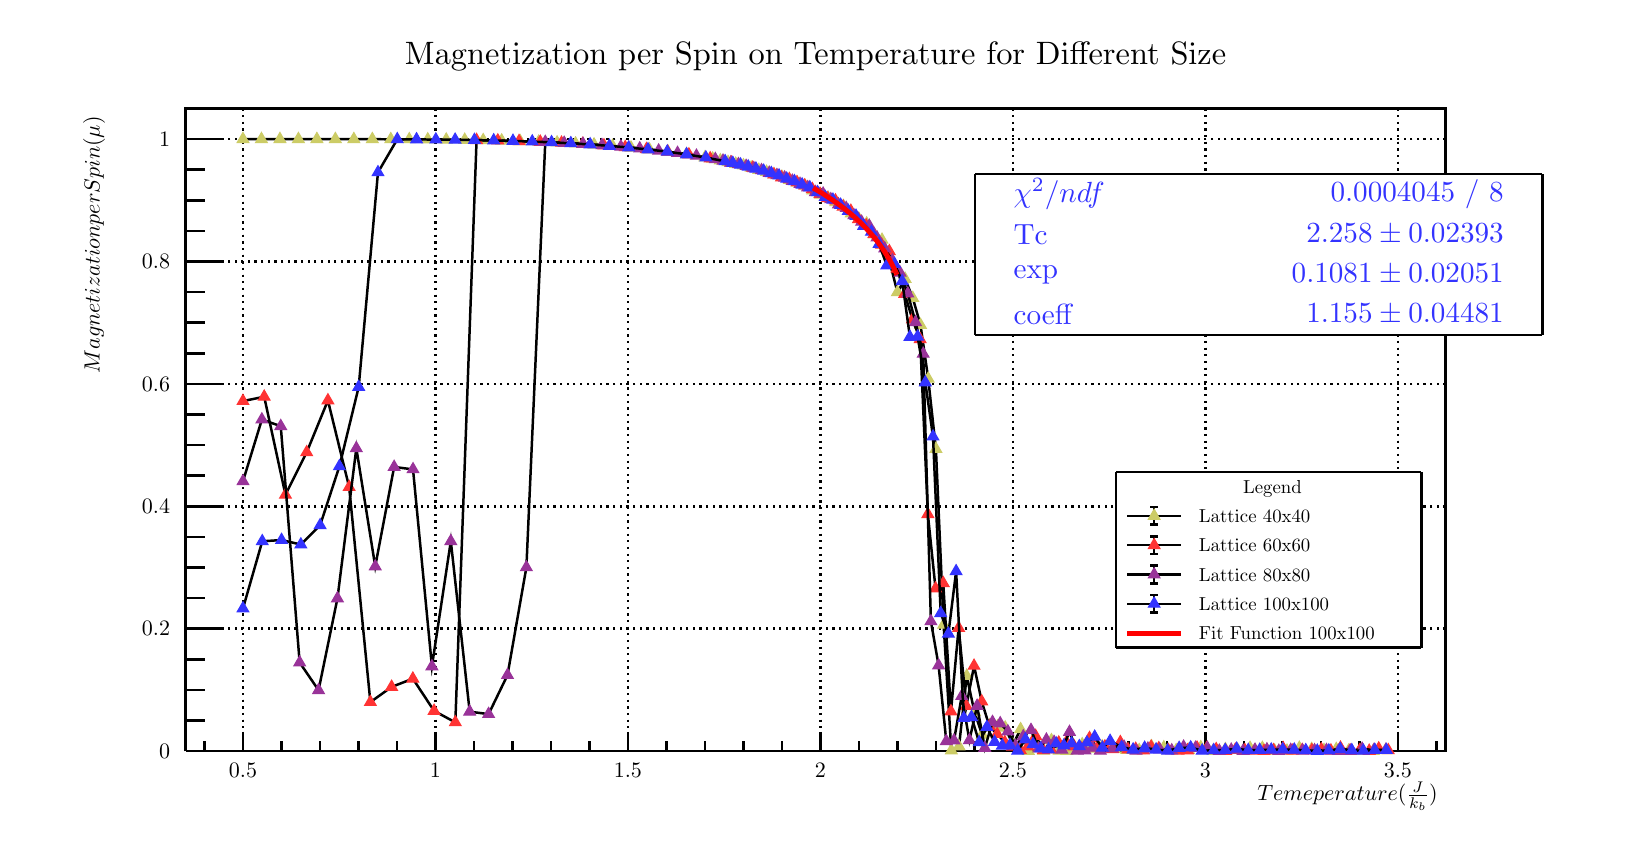
\begin{tikzpicture}
\pgfdeclareplotmark{cross} {
\pgfpathmoveto{\pgfpoint{-0.3\pgfplotmarksize}{\pgfplotmarksize}}
\pgfpathlineto{\pgfpoint{+0.3\pgfplotmarksize}{\pgfplotmarksize}}
\pgfpathlineto{\pgfpoint{+0.3\pgfplotmarksize}{0.3\pgfplotmarksize}}
\pgfpathlineto{\pgfpoint{+1\pgfplotmarksize}{0.3\pgfplotmarksize}}
\pgfpathlineto{\pgfpoint{+1\pgfplotmarksize}{-0.3\pgfplotmarksize}}
\pgfpathlineto{\pgfpoint{+0.3\pgfplotmarksize}{-0.3\pgfplotmarksize}}
\pgfpathlineto{\pgfpoint{+0.3\pgfplotmarksize}{-1.\pgfplotmarksize}}
\pgfpathlineto{\pgfpoint{-0.3\pgfplotmarksize}{-1.\pgfplotmarksize}}
\pgfpathlineto{\pgfpoint{-0.3\pgfplotmarksize}{-0.3\pgfplotmarksize}}
\pgfpathlineto{\pgfpoint{-1.\pgfplotmarksize}{-0.3\pgfplotmarksize}}
\pgfpathlineto{\pgfpoint{-1.\pgfplotmarksize}{0.3\pgfplotmarksize}}
\pgfpathlineto{\pgfpoint{-0.3\pgfplotmarksize}{0.3\pgfplotmarksize}}
\pgfpathclose
\pgfusepathqstroke
}
\pgfdeclareplotmark{cross*} {
\pgfpathmoveto{\pgfpoint{-0.3\pgfplotmarksize}{\pgfplotmarksize}}
\pgfpathlineto{\pgfpoint{+0.3\pgfplotmarksize}{\pgfplotmarksize}}
\pgfpathlineto{\pgfpoint{+0.3\pgfplotmarksize}{0.3\pgfplotmarksize}}
\pgfpathlineto{\pgfpoint{+1\pgfplotmarksize}{0.3\pgfplotmarksize}}
\pgfpathlineto{\pgfpoint{+1\pgfplotmarksize}{-0.3\pgfplotmarksize}}
\pgfpathlineto{\pgfpoint{+0.3\pgfplotmarksize}{-0.3\pgfplotmarksize}}
\pgfpathlineto{\pgfpoint{+0.3\pgfplotmarksize}{-1.\pgfplotmarksize}}
\pgfpathlineto{\pgfpoint{-0.3\pgfplotmarksize}{-1.\pgfplotmarksize}}
\pgfpathlineto{\pgfpoint{-0.3\pgfplotmarksize}{-0.3\pgfplotmarksize}}
\pgfpathlineto{\pgfpoint{-1.\pgfplotmarksize}{-0.3\pgfplotmarksize}}
\pgfpathlineto{\pgfpoint{-1.\pgfplotmarksize}{0.3\pgfplotmarksize}}
\pgfpathlineto{\pgfpoint{-0.3\pgfplotmarksize}{0.3\pgfplotmarksize}}
\pgfpathclose
\pgfusepathqfillstroke
}
\pgfdeclareplotmark{newstar} {
\pgfpathmoveto{\pgfqpoint{0pt}{\pgfplotmarksize}}
\pgfpathlineto{\pgfqpointpolar{44}{0.5\pgfplotmarksize}}
\pgfpathlineto{\pgfqpointpolar{18}{\pgfplotmarksize}}
\pgfpathlineto{\pgfqpointpolar{-20}{0.5\pgfplotmarksize}}
\pgfpathlineto{\pgfqpointpolar{-54}{\pgfplotmarksize}}
\pgfpathlineto{\pgfqpointpolar{-90}{0.5\pgfplotmarksize}}
\pgfpathlineto{\pgfqpointpolar{234}{\pgfplotmarksize}}
\pgfpathlineto{\pgfqpointpolar{198}{0.5\pgfplotmarksize}}
\pgfpathlineto{\pgfqpointpolar{162}{\pgfplotmarksize}}
\pgfpathlineto{\pgfqpointpolar{134}{0.5\pgfplotmarksize}}
\pgfpathclose
\pgfusepathqstroke
}
\pgfdeclareplotmark{newstar*} {
\pgfpathmoveto{\pgfqpoint{0pt}{\pgfplotmarksize}}
\pgfpathlineto{\pgfqpointpolar{44}{0.5\pgfplotmarksize}}
\pgfpathlineto{\pgfqpointpolar{18}{\pgfplotmarksize}}
\pgfpathlineto{\pgfqpointpolar{-20}{0.5\pgfplotmarksize}}
\pgfpathlineto{\pgfqpointpolar{-54}{\pgfplotmarksize}}
\pgfpathlineto{\pgfqpointpolar{-90}{0.5\pgfplotmarksize}}
\pgfpathlineto{\pgfqpointpolar{234}{\pgfplotmarksize}}
\pgfpathlineto{\pgfqpointpolar{198}{0.5\pgfplotmarksize}}
\pgfpathlineto{\pgfqpointpolar{162}{\pgfplotmarksize}}
\pgfpathlineto{\pgfqpointpolar{134}{0.5\pgfplotmarksize}}
\pgfpathclose
\pgfusepathqfillstroke
}
\definecolor{c}{rgb}{1,1,1};
\draw [color=c, fill=c] (0,0) rectangle (20,10.2002);
\draw [color=c, fill=c] (2,1.02002) rectangle (18,9.18019);
\definecolor{c}{rgb}{0,0,0};
\draw [c,line width=0.9] (2,1.02002) -- (2,9.18019) -- (18,9.18019) -- (18,1.02002) -- (2,1.02002);
\definecolor{c}{rgb}{1,1,1};
\draw [color=c, fill=c] (2,1.02002) rectangle (18,9.18019);
\definecolor{c}{rgb}{0,0,0};
\draw [c,line width=0.9] (2,1.02002) -- (2,9.18019) -- (18,9.18019) -- (18,1.02002) -- (2,1.02002);
\draw [c,line width=0.9] (2,1.02002) -- (18,1.02002);
\draw [c,dash pattern=on 0.80pt off 1.60pt ,line width=0.9] (2.72725,9.18019) -- (2.72725,1.02002);
\draw [c,dash pattern=on 0.80pt off 1.60pt ,line width=0.9] (5.17173,9.18019) -- (5.17173,1.02002);
\draw [c,dash pattern=on 0.80pt off 1.60pt ,line width=0.9] (7.61621,9.18019) -- (7.61621,1.02002);
\draw [c,dash pattern=on 0.80pt off 1.60pt ,line width=0.9] (10.0607,9.18019) -- (10.0607,1.02002);
\draw [c,dash pattern=on 0.80pt off 1.60pt ,line width=0.9] (12.5052,9.18019) -- (12.5052,1.02002);
\draw [c,dash pattern=on 0.80pt off 1.60pt ,line width=0.9] (14.9497,9.18019) -- (14.9497,1.02002);
\draw [c,dash pattern=on 0.80pt off 1.60pt ,line width=0.9] (17.3941,9.18019) -- (17.3941,1.02002);
\draw [c,dash pattern=on 0.80pt off 1.60pt ,line width=0.9] (2.72725,9.18019) -- (2.72725,1.02002);
\draw [c,dash pattern=on 0.80pt off 1.60pt ,line width=0.9] (17.3941,9.18019) -- (17.3941,1.02002);
\draw [c,line width=0.9] (2,1.02002) -- (2,9.18019);
\draw [c,dash pattern=on 0.80pt off 1.60pt ,line width=0.9] (18,1.02002) -- (2,1.02002);
\draw [c,dash pattern=on 0.80pt off 1.60pt ,line width=0.9] (18,2.57434) -- (2,2.57434);
\draw [c,dash pattern=on 0.80pt off 1.60pt ,line width=0.9] (18,4.12867) -- (2,4.12867);
\draw [c,dash pattern=on 0.80pt off 1.60pt ,line width=0.9] (18,5.68299) -- (2,5.68299);
\draw [c,dash pattern=on 0.80pt off 1.60pt ,line width=0.9] (18,7.23731) -- (2,7.23731);
\draw [c,dash pattern=on 0.80pt off 1.60pt ,line width=0.9] (18,8.79163) -- (2,8.79163);
\draw [c,dash pattern=on 0.80pt off 1.60pt ,line width=0.9] (18,8.79163) -- (2,8.79163);
\draw [c,line width=0.9] (2,1.02002) -- (18,1.02002);
\draw [c,line width=0.9] (2.72725,1.26483) -- (2.72725,1.02002);
\draw [c,line width=0.9] (3.21614,1.14242) -- (3.21614,1.02002);
\draw [c,line width=0.9] (3.70504,1.14242) -- (3.70504,1.02002);
\draw [c,line width=0.9] (4.19394,1.14242) -- (4.19394,1.02002);
\draw [c,line width=0.9] (4.68283,1.14242) -- (4.68283,1.02002);
\draw [c,line width=0.9] (5.17173,1.26483) -- (5.17173,1.02002);
\draw [c,line width=0.9] (5.66062,1.14242) -- (5.66062,1.02002);
\draw [c,line width=0.9] (6.14952,1.14242) -- (6.14952,1.02002);
\draw [c,line width=0.9] (6.63842,1.14242) -- (6.63842,1.02002);
\draw [c,line width=0.9] (7.12731,1.14242) -- (7.12731,1.02002);
\draw [c,line width=0.9] (7.61621,1.26483) -- (7.61621,1.02002);
\draw [c,line width=0.9] (8.10511,1.14242) -- (8.10511,1.02002);
\draw [c,line width=0.9] (8.594,1.14242) -- (8.594,1.02002);
\draw [c,line width=0.9] (9.0829,1.14242) -- (9.0829,1.02002);
\draw [c,line width=0.9] (9.57179,1.14242) -- (9.57179,1.02002);
\draw [c,line width=0.9] (10.0607,1.26483) -- (10.0607,1.02002);
\draw [c,line width=0.9] (10.5496,1.14242) -- (10.5496,1.02002);
\draw [c,line width=0.9] (11.0385,1.14242) -- (11.0385,1.02002);
\draw [c,line width=0.9] (11.5274,1.14242) -- (11.5274,1.02002);
\draw [c,line width=0.9] (12.0163,1.14242) -- (12.0163,1.02002);
\draw [c,line width=0.9] (12.5052,1.26483) -- (12.5052,1.02002);
\draw [c,line width=0.9] (12.9941,1.14242) -- (12.9941,1.02002);
\draw [c,line width=0.9] (13.483,1.14242) -- (13.483,1.02002);
\draw [c,line width=0.9] (13.9719,1.14242) -- (13.9719,1.02002);
\draw [c,line width=0.9] (14.4608,1.14242) -- (14.4608,1.02002);
\draw [c,line width=0.9] (14.9497,1.26483) -- (14.9497,1.02002);
\draw [c,line width=0.9] (15.4385,1.14242) -- (15.4385,1.02002);
\draw [c,line width=0.9] (15.9274,1.14242) -- (15.9274,1.02002);
\draw [c,line width=0.9] (16.4163,1.14242) -- (16.4163,1.02002);
\draw [c,line width=0.9] (16.9052,1.14242) -- (16.9052,1.02002);
\draw [c,line width=0.9] (17.3941,1.26483) -- (17.3941,1.02002);
\draw [c,line width=0.9] (2.72725,1.26483) -- (2.72725,1.02002);
\draw [c,line width=0.9] (2.23835,1.14242) -- (2.23835,1.02002);
\draw [c,line width=0.9] (17.3941,1.26483) -- (17.3941,1.02002);
\draw [c,line width=0.9] (17.883,1.14242) -- (17.883,1.02002);
\draw [anchor=base] (2.72725,0.683414) node[scale=0.795711, color=c, rotate=0]{0.5};
\draw [anchor=base] (5.17173,0.683414) node[scale=0.795711, color=c, rotate=0]{1};
\draw [anchor=base] (7.61621,0.683414) node[scale=0.795711, color=c, rotate=0]{1.5};
\draw [anchor=base] (10.0607,0.683414) node[scale=0.795711, color=c, rotate=0]{2};
\draw [anchor=base] (12.5052,0.683414) node[scale=0.795711, color=c, rotate=0]{2.5};
\draw [anchor=base] (14.9497,0.683414) node[scale=0.795711, color=c, rotate=0]{3};
\draw [anchor=base] (17.3941,0.683414) node[scale=0.795711, color=c, rotate=0]{3.5};
\draw [anchor= east] (18,0.448809) node[scale=0.795711, color=c, rotate=0]{$Temeperature (\frac{J}{k_{b}})$};
\draw [c,line width=0.9] (2,1.02002) -- (2,9.18019);
\draw [c,line width=0.9] (2.48,1.02002) -- (2,1.02002);
\draw [c,line width=0.9] (2.24,1.4086) -- (2,1.4086);
\draw [c,line width=0.9] (2.24,1.79718) -- (2,1.79718);
\draw [c,line width=0.9] (2.24,2.18576) -- (2,2.18576);
\draw [c,line width=0.9] (2.48,2.57434) -- (2,2.57434);
\draw [c,line width=0.9] (2.24,2.96292) -- (2,2.96292);
\draw [c,line width=0.9] (2.24,3.3515) -- (2,3.3515);
\draw [c,line width=0.9] (2.24,3.74009) -- (2,3.74009);
\draw [c,line width=0.9] (2.48,4.12867) -- (2,4.12867);
\draw [c,line width=0.9] (2.24,4.51725) -- (2,4.51725);
\draw [c,line width=0.9] (2.24,4.90583) -- (2,4.90583);
\draw [c,line width=0.9] (2.24,5.29441) -- (2,5.29441);
\draw [c,line width=0.9] (2.48,5.68299) -- (2,5.68299);
\draw [c,line width=0.9] (2.24,6.07157) -- (2,6.07157);
\draw [c,line width=0.9] (2.24,6.46015) -- (2,6.46015);
\draw [c,line width=0.9] (2.24,6.84873) -- (2,6.84873);
\draw [c,line width=0.9] (2.48,7.23731) -- (2,7.23731);
\draw [c,line width=0.9] (2.24,7.62589) -- (2,7.62589);
\draw [c,line width=0.9] (2.24,8.01447) -- (2,8.01447);
\draw [c,line width=0.9] (2.24,8.40305) -- (2,8.40305);
\draw [c,line width=0.9] (2.48,8.79163) -- (2,8.79163);
\draw [c,line width=0.9] (2.48,8.79163) -- (2,8.79163);
\draw [anchor= east] (1.9,1.02002) node[scale=0.795711, color=c, rotate=0]{0};
\draw [anchor= east] (1.9,2.57434) node[scale=0.795711, color=c, rotate=0]{0.2};
\draw [anchor= east] (1.9,4.12867) node[scale=0.795711, color=c, rotate=0]{0.4};
\draw [anchor= east] (1.9,5.68299) node[scale=0.795711, color=c, rotate=0]{0.6};
\draw [anchor= east] (1.9,7.23731) node[scale=0.795711, color=c, rotate=0]{0.8};
\draw [anchor= east] (1.9,8.79163) node[scale=0.795711, color=c, rotate=0]{1};
\draw [anchor= east] (0.836354,9.18019) node[scale=0.795711, color=c, rotate=90]{$Magnetization per Spin (\mu)$};
\draw [c,line width=0.9] (2.72727,8.79163) -- (2.96195,8.79163) -- (3.19663,8.79161) -- (3.4313,8.79159) -- (3.66598,8.79148) -- (3.90066,8.79133) -- (4.13533,8.79098) -- (4.37001,8.79047) -- (4.60469,8.78979) -- (4.83937,8.78871) --
 (5.07404,8.78699) -- (5.30872,8.78459) -- (5.5434,8.78146) -- (5.77807,8.77738) -- (6.01275,8.77237) -- (6.24743,8.76563) -- (6.4821,8.75733) -- (6.71678,8.74766) -- (6.95146,8.73486) -- (7.18614,8.72133) -- (7.42081,8.70399) -- (7.65549,8.68222) --
 (7.89017,8.65898) -- (8.12484,8.63078) -- (8.35952,8.59938) -- (8.5942,8.55846) -- (8.69198,8.54219) -- (8.78976,8.52113) -- (8.88754,8.49888) -- (8.98531,8.47728) -- (9.08309,8.45732) -- (9.18087,8.4289) -- (9.27865,8.40038) -- (9.37643,8.37424) --
 (9.47421,8.34096) -- (9.57199,8.31186) -- (9.66977,8.27315) -- (9.76755,8.23782) -- (9.86533,8.19924) -- (9.96311,8.13787) -- (10.0609,8.08608) -- (10.1587,8.04633) -- (10.2564,7.9905) -- (10.3542,7.93925) -- (10.452,7.84773) -- (10.5498,7.77827) --
 (10.6476,7.71955) -- (10.7453,7.58049) -- (10.8431,7.51225) -- (10.9409,7.23239) -- (11.0387,6.84736) -- (11.1365,7.01598) -- (11.2342,6.77262) -- (11.332,6.43102) -- (11.4298,5.74798) -- (11.5276,4.85654) -- (11.6254,2.62361) -- (11.7231,1.02795)
 -- (11.8209,1.0783) -- (11.9187,1.97336) -- (12.0165,1.5172) -- (12.1142,1.22757) -- (12.212,1.34693) -- (12.3098,1.331) -- (12.4076,1.3177) -- (12.5054,1.10055) -- (12.6031,1.29689) -- (12.7009,1.02183) -- (12.7987,1.14832) -- (12.8965,1.02444) --
 (12.9943,1.1568) -- (13.092,1.02268) -- (13.1898,1.02002) -- (13.2876,1.03113) -- (13.3854,1.10446) -- (13.4832,1.04863) -- (13.6396,1.07827) -- (13.796,1.0467) -- (13.9525,1.03494) -- (14.1089,1.03099) -- (14.2654,1.08004) -- (14.4218,1.06545) --
 (14.5782,1.02987) -- (14.7347,1.03416) -- (14.8911,1.06775) -- (15.0476,1.02258) -- (15.204,1.04276) -- (15.3604,1.03249) -- (15.5169,1.05935) -- (15.6733,1.05866) -- (15.8298,1.02426) -- (15.9862,1.02297) -- (16.1426,1.05992) -- (16.2991,1.04516)
 -- (16.4555,1.03108) -- (16.612,1.04436) -- (16.7684,1.02421) -- (16.9248,1.02456) -- (17.0813,1.02002) -- (17.2377,1.02964);
\definecolor{c}{rgb}{0.8,0.8,0.4};
\foreach \P in {(2.72727,8.79163), (2.96195,8.79163), (3.19663,8.79161), (3.4313,8.79159), (3.66598,8.79148), (3.90066,8.79133), (4.13533,8.79098), (4.37001,8.79047), (4.60469,8.78979), (4.83937,8.78871), (5.07404,8.78699), (5.30872,8.78459),
 (5.5434,8.78146), (5.77807,8.77738), (6.01275,8.77237), (6.24743,8.76563), (6.4821,8.75733), (6.71678,8.74766), (6.95146,8.73486), (7.18614,8.72133), (7.42081,8.70399), (7.65549,8.68222), (7.89017,8.65898), (8.12484,8.63078), (8.35952,8.59938),
 (8.5942,8.55846), (8.69198,8.54219), (8.78976,8.52113), (8.88754,8.49888), (8.98531,8.47728), (9.08309,8.45732), (9.18087,8.4289), (9.27865,8.40038), (9.37643,8.37424), (9.47421,8.34096), (9.57199,8.31186), (9.66977,8.27315), (9.76755,8.23782),
 (9.86533,8.19924), (9.96311,8.13787), (10.0609,8.08608), (10.1587,8.04633), (10.2564,7.9905), (10.3542,7.93925), (10.452,7.84773), (10.5498,7.77827), (10.6476,7.71955), (10.7453,7.58049), (10.8431,7.51225), (10.9409,7.23239), (11.0387,6.84736),
 (11.1365,7.01598), (11.2342,6.77262), (11.332,6.43102), (11.4298,5.74798), (11.5276,4.85654), (11.6254,2.62361), (11.7231,1.02795), (11.8209,1.0783), (11.9187,1.97336), (12.0165,1.5172), (12.1142,1.22757), (12.212,1.34693), (12.3098,1.331),
 (12.4076,1.3177), (12.5054,1.10055), (12.6031,1.29689), (12.7009,1.02183), (12.7987,1.14832), (12.8965,1.02444), (12.9943,1.1568), (13.092,1.02268), (13.1898,1.02036), (13.2876,1.03113), (13.3854,1.10446), (13.4832,1.04863), (13.6396,1.07827),
 (13.796,1.0467), (13.9525,1.03494), (14.1089,1.03099), (14.2654,1.08004), (14.4218,1.06545), (14.5782,1.02987), (14.7347,1.03416), (14.8911,1.06775), (15.0476,1.02258), (15.204,1.04276), (15.3604,1.03249), (15.5169,1.05935), (15.6733,1.05866),
 (15.8298,1.02426), (15.9862,1.02297), (16.1426,1.05992), (16.2991,1.04516), (16.4555,1.03108), (16.612,1.04436), (16.7684,1.02421), (16.9248,1.02456), (17.0813,1.0208), (17.2377,1.02964)}{\draw[mark options={color=c,fill=c},mark
 size=2.402402pt,mark=triangle*] plot coordinates {\P};}
\definecolor{c}{rgb}{0,0,0};
\draw [c,line width=0.9] (2.72727,5.46474) -- (2.99696,5.52007) -- (3.26665,4.27547) -- (3.53634,4.81398) -- (3.80603,5.47331) -- (4.07572,4.37265) -- (4.34541,1.64192) -- (4.61509,1.83503) -- (4.88478,1.93927) -- (5.15447,1.53034) --
 (5.42416,1.38475) -- (5.69385,8.77886) -- (5.96354,8.77358) -- (6.23323,8.76577) -- (6.50292,8.75659) -- (6.7726,8.74452) -- (7.04229,8.7303) -- (7.31198,8.71126) -- (7.58167,8.68885) -- (7.85136,8.66324) -- (8.12105,8.63133) -- (8.39074,8.59562) --
 (8.66043,8.54592) -- (8.93012,8.49248) -- (9.1998,8.42721) -- (9.46949,8.3428) -- (9.56727,8.30384) -- (9.66505,8.28272) -- (9.76283,8.2428) -- (9.86061,8.20158) -- (9.95839,8.15604) -- (10.0562,8.09539) -- (10.1539,8.04066) -- (10.2517,8.01143) --
 (10.3495,7.93399) -- (10.4473,7.87944) -- (10.5451,7.77476) -- (10.6428,7.69386) -- (10.7406,7.58528) -- (10.8384,7.45108) -- (10.9362,7.36707) -- (11.034,7.14479) -- (11.1317,6.82595) -- (11.2295,6.50116) -- (11.3273,6.24988) -- (11.4251,4.0292) --
 (11.5229,3.08461) -- (11.6206,3.15274) -- (11.7184,1.52299) -- (11.8162,2.58373) -- (11.914,1.59122) -- (12.0118,2.10213) -- (12.1095,1.64945) -- (12.2073,1.33349) -- (12.3051,1.2368) -- (12.4029,1.1303) -- (12.5006,1.07605) -- (12.5984,1.03225) --
 (12.6962,1.07834) -- (12.794,1.2107) -- (12.8918,1.03053) -- (12.9895,1.03881) -- (13.0873,1.12682) -- (13.1851,1.13427) -- (13.2829,1.07951) -- (13.3807,1.05115) -- (13.4784,1.18412) -- (13.5762,1.06496) -- (13.674,1.07725) -- (13.7718,1.04437) --
 (13.8696,1.13231) -- (13.9673,1.04159) -- (14.0651,1.04693) -- (14.1629,1.0277) -- (14.2607,1.0741) -- (14.3585,1.05509) -- (14.4799,1.03152) -- (14.6013,1.02576) -- (14.7227,1.02867) -- (14.8442,1.06163) -- (14.9656,1.05523) -- (15.087,1.0432) --
 (15.2085,1.02002) -- (15.3299,1.03612) -- (15.4513,1.02941) -- (15.5727,1.02318) -- (15.6942,1.02002) -- (15.8156,1.03005) -- (15.937,1.05714) -- (16.0584,1.02367) -- (16.1799,1.03196) -- (16.3013,1.03024) -- (16.4227,1.04099) -- (16.5442,1.02503)
 -- (16.6656,1.06197) -- (16.787,1.02601) -- (16.9084,1.02948) -- (17.0299,1.02255) -- (17.1513,1.05175) -- (17.2727,1.02903);
\definecolor{c}{rgb}{1,0.2,0.2};
\foreach \P in {(2.72727,5.46474), (2.99696,5.52007), (3.26665,4.27547), (3.53634,4.81398), (3.80603,5.47331), (4.07572,4.37265), (4.34541,1.64192), (4.61509,1.83503), (4.88478,1.93927), (5.15447,1.53034), (5.42416,1.38475), (5.69385,8.77886),
 (5.96354,8.77358), (6.23323,8.76577), (6.50292,8.75659), (6.7726,8.74452), (7.04229,8.7303), (7.31198,8.71126), (7.58167,8.68885), (7.85136,8.66324), (8.12105,8.63133), (8.39074,8.59562), (8.66043,8.54592), (8.93012,8.49248), (9.1998,8.42721),
 (9.46949,8.3428), (9.56727,8.30384), (9.66505,8.28272), (9.76283,8.2428), (9.86061,8.20158), (9.95839,8.15604), (10.0562,8.09539), (10.1539,8.04066), (10.2517,8.01143), (10.3495,7.93399), (10.4473,7.87944), (10.5451,7.77476), (10.6428,7.69386),
 (10.7406,7.58528), (10.8384,7.45108), (10.9362,7.36707), (11.034,7.14479), (11.1317,6.82595), (11.2295,6.50116), (11.3273,6.24988), (11.4251,4.0292), (11.5229,3.08461), (11.6206,3.15274), (11.7184,1.52299), (11.8162,2.58373), (11.914,1.59122),
 (12.0118,2.10213), (12.1095,1.64945), (12.2073,1.33349), (12.3051,1.2368), (12.4029,1.1303), (12.5006,1.07605), (12.5984,1.03225), (12.6962,1.07834), (12.794,1.2107), (12.8918,1.03053), (12.9895,1.03881), (13.0873,1.12682), (13.1851,1.13427),
 (13.2829,1.07951), (13.3807,1.05115), (13.4784,1.18412), (13.5762,1.06496), (13.674,1.07725), (13.7718,1.04437), (13.8696,1.13231), (13.9673,1.04159), (14.0651,1.04693), (14.1629,1.0277), (14.2607,1.0741), (14.3585,1.05509), (14.4799,1.03152),
 (14.6013,1.02576), (14.7227,1.02867), (14.8442,1.06163), (14.9656,1.05523), (15.087,1.0432), (15.2085,1.02071), (15.3299,1.03612), (15.4513,1.02941), (15.5727,1.02318), (15.6942,1.02041), (15.8156,1.03005), (15.937,1.05714), (16.0584,1.02367),
 (16.1799,1.03196), (16.3013,1.03024), (16.4227,1.04099), (16.5442,1.02503), (16.6656,1.06197), (16.787,1.02601), (16.9084,1.02948), (17.0299,1.02255), (17.1513,1.05175), (17.2727,1.02903)}{\draw[mark options={color=c,fill=c},mark
 size=2.402402pt,mark=triangle*] plot coordinates {\P};}
\definecolor{c}{rgb}{0,0,0};
\draw [c,line width=0.9] (2.72727,4.44613) -- (2.96723,5.23055) -- (3.20718,5.14589) -- (3.44714,2.14455) -- (3.68709,1.793) -- (3.92705,2.95908) -- (4.167,4.86524) -- (4.40695,3.3651) -- (4.64691,4.62793) -- (4.88686,4.59773) -- (5.12682,2.09567) --
 (5.36677,3.68493) -- (5.60673,1.5203) -- (5.84668,1.48964) -- (6.08664,1.98487) -- (6.32659,3.35338) -- (6.56655,8.7544) -- (6.8065,8.74301) -- (7.04645,8.7297) -- (7.28641,8.7138) -- (7.52636,8.69539) -- (7.76632,8.67253) -- (8.00627,8.64527) --
 (8.24623,8.6149) -- (8.48618,8.5795) -- (8.72614,8.53675) -- (8.82391,8.51623) -- (8.92169,8.4932) -- (9.01947,8.47248) -- (9.11725,8.44934) -- (9.21503,8.42142) -- (9.31281,8.39585) -- (9.41059,8.36306) -- (9.50837,8.3332) -- (9.60615,8.30244) --
 (9.70393,8.26052) -- (9.80171,8.22176) -- (9.89949,8.17883) -- (9.99726,8.11757) -- (10.095,8.09779) -- (10.1928,8.02707) -- (10.2906,7.96138) -- (10.3884,7.91559) -- (10.4862,7.82347) -- (10.5839,7.74102) -- (10.6817,7.68976) -- (10.7795,7.54109)
 -- (10.8773,7.40163) -- (10.9751,7.25074) -- (11.0728,7.095) -- (11.1706,6.82981) -- (11.2684,6.46612) -- (11.3662,6.0649) -- (11.464,2.66728) -- (11.5617,2.10709) -- (11.6595,1.14478) -- (11.7573,1.15411) -- (11.8551,1.71861) -- (11.9528,1.15789)
 -- (12.0506,1.59308) -- (12.1484,1.05936) -- (12.2462,1.38797) -- (12.344,1.37128) -- (12.4417,1.26831) -- (12.5395,1.08599) -- (12.6373,1.20591) -- (12.7351,1.2865) -- (12.8329,1.05163) -- (12.9306,1.16399) -- (13.0284,1.13418) -- (13.1262,1.03706)
 -- (13.224,1.2617) -- (13.3218,1.02544) -- (13.4195,1.02847) -- (13.5173,1.06208) -- (13.6151,1.02498) -- (13.7663,1.05376) -- (13.9174,1.07274) -- (14.0686,1.02446) -- (14.2197,1.05007) -- (14.3709,1.03905) -- (14.5221,1.02783) -- (14.6732,1.07445)
 -- (14.8244,1.06033) -- (14.9756,1.05996) -- (15.1267,1.02227) -- (15.2779,1.03593) -- (15.429,1.0222) -- (15.5802,1.03482) -- (15.7314,1.04015) -- (15.8825,1.02196) -- (16.0337,1.03288) -- (16.1849,1.02438) -- (16.336,1.02876) -- (16.4872,1.03074)
 -- (16.6383,1.02088) -- (16.7895,1.02222) -- (16.9407,1.04665) -- (17.0918,1.03423) -- (17.243,1.03519);
\definecolor{c}{rgb}{0.6,0.2,0.6};
\foreach \P in {(2.72727,4.44613), (2.96723,5.23055), (3.20718,5.14589), (3.44714,2.14455), (3.68709,1.793), (3.92705,2.95908), (4.167,4.86524), (4.40695,3.3651), (4.64691,4.62793), (4.88686,4.59773), (5.12682,2.09567), (5.36677,3.68493),
 (5.60673,1.5203), (5.84668,1.48964), (6.08664,1.98487), (6.32659,3.35338), (6.56655,8.7544), (6.8065,8.74301), (7.04645,8.7297), (7.28641,8.7138), (7.52636,8.69539), (7.76632,8.67253), (8.00627,8.64527), (8.24623,8.6149), (8.48618,8.5795),
 (8.72614,8.53675), (8.82391,8.51623), (8.92169,8.4932), (9.01947,8.47248), (9.11725,8.44934), (9.21503,8.42142), (9.31281,8.39585), (9.41059,8.36306), (9.50837,8.3332), (9.60615,8.30244), (9.70393,8.26052), (9.80171,8.22176), (9.89949,8.17883),
 (9.99726,8.11757), (10.095,8.09779), (10.1928,8.02707), (10.2906,7.96138), (10.3884,7.91559), (10.4862,7.82347), (10.5839,7.74102), (10.6817,7.68976), (10.7795,7.54109), (10.8773,7.40163), (10.9751,7.25074), (11.0728,7.095), (11.1706,6.82981),
 (11.2684,6.46612), (11.3662,6.0649), (11.464,2.66728), (11.5617,2.10709), (11.6595,1.14478), (11.7573,1.15411), (11.8551,1.71861), (11.9528,1.15789), (12.0506,1.59308), (12.1484,1.05936), (12.2462,1.38797), (12.344,1.37128), (12.4417,1.26831),
 (12.5395,1.08599), (12.6373,1.20591), (12.7351,1.2865), (12.8329,1.05163), (12.9306,1.16399), (13.0284,1.13418), (13.1262,1.03706), (13.224,1.2617), (13.3218,1.02544), (13.4195,1.02847), (13.5173,1.06208), (13.6151,1.02498), (13.7663,1.05376),
 (13.9174,1.07274), (14.0686,1.02446), (14.2197,1.05007), (14.3709,1.03905), (14.5221,1.02783), (14.6732,1.07445), (14.8244,1.06033), (14.9756,1.05996), (15.1267,1.02227), (15.2779,1.03593), (15.429,1.0222), (15.5802,1.03482), (15.7314,1.04015),
 (15.8825,1.02196), (16.0337,1.03288), (16.1849,1.02438), (16.336,1.02876), (16.4872,1.03074), (16.6383,1.02088), (16.7895,1.02222), (16.9407,1.04665), (17.0918,1.03423), (17.243,1.03519)}{\draw[mark options={color=c,fill=c},mark
 size=2.402402pt,mark=triangle*] plot coordinates {\P};}
\definecolor{c}{rgb}{1,1,1};
\draw [color=c, fill=c] (12.0232,6.30538) rectangle (19.2308,8.34766);
\definecolor{c}{rgb}{0,0,0};
\draw [c,line width=0.9] (12.0232,6.30538) -- (18,6.30538);
\draw [c,line width=0.9] (18,8.34766) -- (12.0232,8.34766);
\draw [c,line width=0.9] (12.0232,8.34766) -- (12.0232,6.30538);
\definecolor{c}{rgb}{0.2,0.2,1};
\draw [anchor= west] (12.3836,8.09237) node[scale=1.05315, color=c, rotate=0]{$\chi^{2} / ndf $};
\draw [anchor= east] (18.8704,8.09237) node[scale=1.05315, color=c, rotate=0]{ 0.0004045 / 8};
\draw [anchor= west] (12.3836,7.5818) node[scale=1.05315, color=c, rotate=0]{Tc       };
\draw [anchor= east] (18.8704,7.5818) node[scale=1.05315, color=c, rotate=0]{$ 2.258 \pm 0.02393$};
\draw [anchor= west] (12.3836,7.07123) node[scale=1.05315, color=c, rotate=0]{exp      };
\draw [anchor= east] (18.8704,7.07123) node[scale=1.05315, color=c, rotate=0]{$ 0.1081 \pm 0.02051$};
\draw [anchor= west] (12.3836,6.56067) node[scale=1.05315, color=c, rotate=0]{coeff    };
\draw [anchor= east] (18.8704,6.56067) node[scale=1.05315, color=c, rotate=0]{$ 1.155 \pm 0.04481$};
\definecolor{c}{rgb}{0,0,0};
\draw [c,line width=0.9] (2.72727,2.83128) -- (2.97221,3.68435) -- (3.21714,3.70018) -- (3.46207,3.64313) -- (3.70701,3.88756) -- (3.95194,4.63583) -- (4.19687,5.64437) -- (4.4418,8.36951) -- (4.68674,8.78936) -- (4.93167,8.788) -- (5.1766,8.78588)
 -- (5.42154,8.78314) -- (5.66647,8.77956) -- (5.9114,8.77452) -- (6.15634,8.76861) -- (6.40127,8.76039) -- (6.6462,8.75089) -- (6.89114,8.7381) -- (7.13607,8.72415) -- (7.381,8.70578) -- (7.62593,8.68556) -- (7.87087,8.66052) -- (8.1158,8.63258) --
 (8.36073,8.59774) -- (8.60567,8.55744) -- (8.8506,8.50966) -- (8.94838,8.48734) -- (9.04616,8.46704) -- (9.14394,8.44212) -- (9.24172,8.41596) -- (9.3395,8.38865) -- (9.43727,8.35866) -- (9.53505,8.32849) -- (9.63283,8.28726) -- (9.73061,8.25586) --
 (9.82839,8.21379) -- (9.92617,8.17753) -- (10.024,8.11607) -- (10.1217,8.05628) -- (10.2195,8.02062) -- (10.3173,7.95531) -- (10.4151,7.87922) -- (10.5128,7.81676) -- (10.6106,7.68997) -- (10.7084,7.61385) -- (10.8062,7.46007) -- (10.904,7.18786) --
 (11.0017,7.20458) -- (11.0995,6.9876) -- (11.1973,6.27901) -- (11.2951,6.28302) -- (11.3929,5.70148) -- (11.4906,5.01423) -- (11.5884,2.7711) -- (11.6862,2.51017) -- (11.784,3.30316) -- (11.8818,1.43892) -- (11.9795,1.45072) -- (12.0773,1.13079) --
 (12.1751,1.32488) -- (12.2729,1.13527) -- (12.3707,1.08758) -- (12.4684,1.09484) -- (12.5662,1.02449) -- (12.664,1.16796) -- (12.7618,1.10703) -- (12.8595,1.05309) -- (12.9573,1.03921) -- (13.0551,1.11487) -- (13.1529,1.09078) -- (13.2507,1.11557)
 -- (13.3484,1.08034) -- (13.4462,1.12778) -- (13.544,1.20065) -- (13.6418,1.06258) -- (13.7396,1.14758) -- (13.8857,1.07) -- (14.0319,1.03828) -- (14.1781,1.06) -- (14.3243,1.03828) -- (14.4705,1.02549) -- (14.6167,1.05856) -- (14.7628,1.06484) --
 (14.909,1.02491) -- (15.0552,1.03013) -- (15.2014,1.03318) -- (15.3476,1.04878) -- (15.4938,1.03103) -- (15.6399,1.0338) -- (15.7861,1.03744) -- (15.9323,1.04059) -- (16.0785,1.03744) -- (16.2247,1.02985) -- (16.3709,1.02252) -- (16.5171,1.02599) --
 (16.6632,1.04503) -- (16.8094,1.0299) -- (16.9556,1.02322) -- (17.1018,1.03216) -- (17.248,1.03245);
\definecolor{c}{rgb}{0.2,0.2,1};
\foreach \P in {(2.72727,2.83128), (2.97221,3.68435), (3.21714,3.70018), (3.46207,3.64313), (3.70701,3.88756), (3.95194,4.63583), (4.19687,5.64437), (4.4418,8.36951), (4.68674,8.78936), (4.93167,8.788), (5.1766,8.78588), (5.42154,8.78314),
 (5.66647,8.77956), (5.9114,8.77452), (6.15634,8.76861), (6.40127,8.76039), (6.6462,8.75089), (6.89114,8.7381), (7.13607,8.72415), (7.381,8.70578), (7.62593,8.68556), (7.87087,8.66052), (8.1158,8.63258), (8.36073,8.59774), (8.60567,8.55744),
 (8.8506,8.50966), (8.94838,8.48734), (9.04616,8.46704), (9.14394,8.44212), (9.24172,8.41596), (9.3395,8.38865), (9.43727,8.35866), (9.53505,8.32849), (9.63283,8.28726), (9.73061,8.25586), (9.82839,8.21379), (9.92617,8.17753), (10.024,8.11607),
 (10.1217,8.05628), (10.2195,8.02062), (10.3173,7.95531), (10.4151,7.87922), (10.5128,7.81676), (10.6106,7.68997), (10.7084,7.61385), (10.8062,7.46007), (10.904,7.18786), (11.0017,7.20458), (11.0995,6.9876), (11.1973,6.27901), (11.2951,6.28302),
 (11.3929,5.70148), (11.4906,5.01423), (11.5884,2.7711), (11.6862,2.51017), (11.784,3.30316), (11.8818,1.43892), (11.9795,1.45072), (12.0773,1.13079), (12.1751,1.32488), (12.2729,1.13527), (12.3707,1.08758), (12.4684,1.09484), (12.5662,1.02449),
 (12.664,1.16796), (12.7618,1.10703), (12.8595,1.05309), (12.9573,1.03921), (13.0551,1.11487), (13.1529,1.09078), (13.2507,1.11557), (13.3484,1.08034), (13.4462,1.12778), (13.544,1.20065), (13.6418,1.06258), (13.7396,1.14758), (13.8857,1.07),
 (14.0319,1.03828), (14.1781,1.06), (14.3243,1.03828), (14.4705,1.02549), (14.6167,1.05856), (14.7628,1.06484), (14.909,1.02491), (15.0552,1.03013), (15.2014,1.03318), (15.3476,1.04878), (15.4938,1.03103), (15.6399,1.0338), (15.7861,1.03744),
 (15.9323,1.04059), (16.0785,1.03744), (16.2247,1.02985), (16.3709,1.02252), (16.5171,1.02599), (16.6632,1.04503), (16.8094,1.0299), (16.9556,1.02322), (17.1018,1.03216), (17.248,1.03245)}{\draw[mark options={color=c,fill=c},mark
 size=2.402402pt,mark=triangle*] plot coordinates {\P};}
\definecolor{c}{rgb}{1,0,0};
\draw [c,line width=1.8] (9.96829,8.1716) -- (9.97904,8.16542) -- (9.9898,8.15921) -- (10.0006,8.15295) -- (10.0113,8.14664) -- (10.0221,8.14029) -- (10.0328,8.13389) -- (10.0436,8.12744) -- (10.0543,8.12094) -- (10.0651,8.1144) -- (10.0758,8.1078)
 -- (10.0866,8.10115) -- (10.0974,8.09446) -- (10.1081,8.0877) -- (10.1189,8.0809) -- (10.1296,8.07404) -- (10.1404,8.06712) -- (10.1511,8.06015) -- (10.1619,8.05312) -- (10.1726,8.04603) -- (10.1834,8.03889) -- (10.1942,8.03168) -- (10.2049,8.02441)
 -- (10.2157,8.01707) -- (10.2264,8.00968) -- (10.2372,8.00222) -- (10.2479,7.99469) -- (10.2587,7.98709) -- (10.2694,7.97943) -- (10.2802,7.97169) -- (10.291,7.96388) -- (10.3017,7.95601) -- (10.3125,7.94805) -- (10.3232,7.94002) -- (10.334,7.93191)
 -- (10.3447,7.92372) -- (10.3555,7.91546) -- (10.3663,7.9071) -- (10.377,7.89867) -- (10.3878,7.89015) -- (10.3985,7.88154) -- (10.4093,7.87284) -- (10.42,7.86404) -- (10.4308,7.85516) -- (10.4415,7.84618) -- (10.4523,7.83709) -- (10.4631,7.82791)
 -- (10.4738,7.81863) -- (10.4846,7.80923) -- (10.4953,7.79973);
\draw [c,line width=1.8] (10.4953,7.79973) -- (10.5061,7.79012) -- (10.5168,7.7804) -- (10.5276,7.77056) -- (10.5383,7.76059) -- (10.5491,7.75051) -- (10.5599,7.7403) -- (10.5706,7.72996) -- (10.5814,7.71948) -- (10.5921,7.70887) -- (10.6029,7.69812)
 -- (10.6136,7.68722) -- (10.6244,7.67618) -- (10.6351,7.66498) -- (10.6459,7.65362) -- (10.6567,7.6421) -- (10.6674,7.63041) -- (10.6782,7.61855) -- (10.6889,7.60651) -- (10.6997,7.59429) -- (10.7104,7.58187) -- (10.7212,7.56926) --
 (10.7319,7.55645) -- (10.7427,7.54342) -- (10.7535,7.53018) -- (10.7642,7.51671) -- (10.775,7.503) -- (10.7857,7.48905) -- (10.7965,7.47485) -- (10.8072,7.46039) -- (10.818,7.44565) -- (10.8287,7.43063) -- (10.8395,7.41532) -- (10.8503,7.39969) --
 (10.861,7.38374) -- (10.8718,7.36746) -- (10.8825,7.35082) -- (10.8933,7.33381) -- (10.904,7.31642) -- (10.9148,7.29862) -- (10.9255,7.28039) -- (10.9363,7.26172) -- (10.9471,7.24257) -- (10.9578,7.22293) -- (10.9686,7.20275) -- (10.9793,7.18202) --
 (10.9901,7.1607) -- (11.0008,7.13875) -- (11.0116,7.11612) -- (11.0223,7.09278);
\draw [c,line width=1.8] (11.0223,7.09278) -- (11.0331,7.06868);
\definecolor{c}{rgb}{1,1,1};
\draw [color=c, fill=c] (12.0232,6.30538) rectangle (19.2308,8.34766);
\definecolor{c}{rgb}{0,0,0};
\draw [c,line width=0.9] (12.0232,6.30538) -- (19.2308,6.30538);
\draw [c,line width=0.9] (19.2308,6.30538) -- (19.2308,8.34766);
\draw [c,line width=0.9] (19.2308,8.34766) -- (12.0232,8.34766);
\draw [c,line width=0.9] (12.0232,8.34766) -- (12.0232,6.30538);
\definecolor{c}{rgb}{0.2,0.2,1};
\draw [anchor= west] (12.3836,8.09237) node[scale=1.05315, color=c, rotate=0]{$\chi^{2} / ndf $};
\draw [anchor= east] (18.8704,8.09237) node[scale=1.05315, color=c, rotate=0]{ 0.0004045 / 8};
\draw [anchor= west] (12.3836,7.5818) node[scale=1.05315, color=c, rotate=0]{Tc       };
\draw [anchor= east] (18.8704,7.5818) node[scale=1.05315, color=c, rotate=0]{$ 2.258 \pm 0.02393$};
\draw [anchor= west] (12.3836,7.07123) node[scale=1.05315, color=c, rotate=0]{exp      };
\draw [anchor= east] (18.8704,7.07123) node[scale=1.05315, color=c, rotate=0]{$ 0.1081 \pm 0.02051$};
\draw [anchor= west] (12.3836,6.56067) node[scale=1.05315, color=c, rotate=0]{coeff    };
\draw [anchor= east] (18.8704,6.56067) node[scale=1.05315, color=c, rotate=0]{$ 1.155 \pm 0.04481$};
\definecolor{c}{rgb}{0,0,0};
\draw (10,9.83933) node[scale=1.17016, color=c, rotate=0]{Magnetization per Spin on Temperature for Different Size};
\definecolor{c}{rgb}{1,1,1};
\draw [color=c, fill=c] (13.8145,2.33243) rectangle (17.6923,4.56443);
\definecolor{c}{rgb}{0,0,0};
\draw [c,line width=0.9] (13.8145,2.33243) -- (17.6923,2.33243);
\draw [c,line width=0.9] (17.6923,2.33243) -- (17.6923,4.56443);
\draw [c,line width=0.9] (17.6923,4.56443) -- (13.8145,4.56443);
\draw [c,line width=0.9] (13.8145,4.56443) -- (13.8145,2.33243);
\draw [anchor=base] (15.8019,4.29473) node[scale=0.678695, color=c, rotate=0]{Legend};
\draw [anchor=base west] (14.784,3.92273) node[scale=0.678695, color=c, rotate=0]{Lattice 40x40};
\draw [c,line width=0.9] (13.96,4.00643) -- (14.6386,4.00643);
\draw [c,line width=0.9] (14.2993,4.04858) -- (14.2993,4.11803);
\draw [c,line width=0.9] (14.2993,3.96428) -- (14.2993,3.89483);
\draw [c,line width=0.9] (14.2484,4.11803) -- (14.3502,4.11803);
\draw [c,line width=0.9] (14.2484,3.89483) -- (14.3502,3.89483);
\definecolor{c}{rgb}{0.8,0.8,0.4};
\foreach \P in {(14.2993,4.00643)}{\draw[mark options={color=c,fill=c},mark size=2.402402pt,mark=triangle*] plot coordinates {\P};}
\definecolor{c}{rgb}{0,0,0};
\draw [anchor=base west] (14.784,3.55073) node[scale=0.678695, color=c, rotate=0]{Lattice 60x60};
\draw [c,line width=0.9] (13.96,3.63443) -- (14.6386,3.63443);
\draw [c,line width=0.9] (14.2993,3.67658) -- (14.2993,3.74603);
\draw [c,line width=0.9] (14.2993,3.59228) -- (14.2993,3.52283);
\draw [c,line width=0.9] (14.2484,3.74603) -- (14.3502,3.74603);
\draw [c,line width=0.9] (14.2484,3.52283) -- (14.3502,3.52283);
\definecolor{c}{rgb}{1,0.2,0.2};
\foreach \P in {(14.2993,3.63443)}{\draw[mark options={color=c,fill=c},mark size=2.402402pt,mark=triangle*] plot coordinates {\P};}
\definecolor{c}{rgb}{0,0,0};
\draw [anchor=base west] (14.784,3.17873) node[scale=0.678695, color=c, rotate=0]{Lattice 80x80};
\draw [c,line width=0.9] (13.96,3.26243) -- (14.6386,3.26243);
\draw [c,line width=0.9] (14.2993,3.30458) -- (14.2993,3.37403);
\draw [c,line width=0.9] (14.2993,3.22028) -- (14.2993,3.15083);
\draw [c,line width=0.9] (14.2484,3.37403) -- (14.3502,3.37403);
\draw [c,line width=0.9] (14.2484,3.15083) -- (14.3502,3.15083);
\definecolor{c}{rgb}{0.6,0.2,0.6};
\foreach \P in {(14.2993,3.26243)}{\draw[mark options={color=c,fill=c},mark size=2.402402pt,mark=triangle*] plot coordinates {\P};}
\definecolor{c}{rgb}{0,0,0};
\draw [anchor=base west] (14.784,2.80673) node[scale=0.678695, color=c, rotate=0]{Lattice 100x100};
\draw [c,line width=0.9] (13.96,2.89043) -- (14.6386,2.89043);
\draw [c,line width=0.9] (14.2993,2.93258) -- (14.2993,3.00203);
\draw [c,line width=0.9] (14.2993,2.84828) -- (14.2993,2.77883);
\draw [c,line width=0.9] (14.2484,3.00203) -- (14.3502,3.00203);
\draw [c,line width=0.9] (14.2484,2.77883) -- (14.3502,2.77883);
\definecolor{c}{rgb}{0.2,0.2,1};
\foreach \P in {(14.2993,2.89043)}{\draw[mark options={color=c,fill=c},mark size=2.402402pt,mark=triangle*] plot coordinates {\P};}
\definecolor{c}{rgb}{0,0,0};
\draw [anchor=base west] (14.784,2.43473) node[scale=0.678695, color=c, rotate=0]{Fit Function 100x100};
\definecolor{c}{rgb}{1,0,0};
\draw [c,line width=1.8] (13.96,2.51843) -- (14.6386,2.51843);
\end{tikzpicture}
